\section{Mateusz Działowski}
\label{sec:Mateusz Działowski}
 
\subsection{Wyrażanie matematyczne} \[\int_0^1 x^2 dx = \frac{1}{3}\)

\subsection{Zdjęcie}
\begin{figure}[htbp]
    \centering
    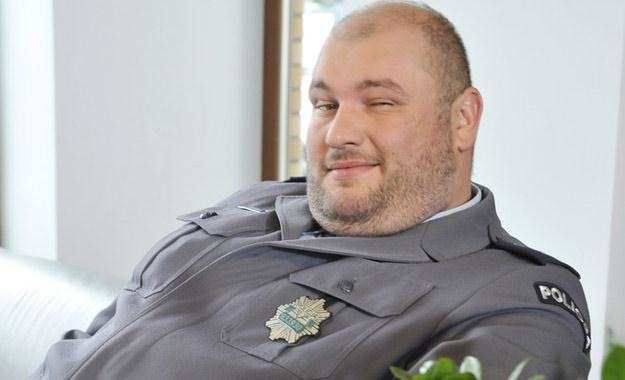
\includegraphics[scale= 0.5]{pictures/nocul.jpg}
    \caption{To jest Mietek Nocul.}
    \label{fig:nocul}
\end{figure}

\subsection{Tabela}
Tabela przedstawia losowe imiona i nazwiska.
\label{tab}
\begin{table}[h]
\begin{tabular}{|l|l|l|ll}
\cline{1-3}
Imię   & Nazwisko & Wiek &  &  \\ \cline{1-3}
Paweł  & Kępa     & 12   &  &  \\ \cline{1-3}
Konrad & Rybik    & 41   &  &  \\ \cline{1-3}
Rafał  & Bomba    & 52   &  &  \\ \cline{1-3}
\end{tabular}
\end{table}

\subsection{Listy}
\textbf{Imiona}
\begin{itemize}
    \item Mateusz
    \item Paweł
    \item Szymon
\end{itemize}

\textbf{Ćwiczenia}
\begin{enumerate}
    \item Podciąganie
    \item Pompki
    \item Przysiady
    \item Dipy
\end{enumerate}

\subsection{Tekst}
To jest \textbf{tekst pogrubiony} oraz \textit{kursywa}.\\
Ten tekst jest \underline{podkreślony}.
